\documentclass[12pt]{article}

% custom commands
\newcommand{\paren}[1]{\left( {#1} \right)}
\newcommand{\abs}[1]{\left| {#1} \right|}

% Math and symbol packages
\usepackage{amsmath}
\usepackage{amssymb}
\usepackage{derivative}

% Figure Packages
\usepackage{graphicx}
\usepackage{wrapfig}
\usepackage{epstopdf}
\usepackage{float}
\usepackage{subfigure}

% Formatting and Random Text Generation
\usepackage{inputenc}
\usepackage[left=2.54cm,right=2.54cm,top=2.54cm,bottom=2.54cm]{geometry}
\usepackage{lipsum}

% Header and indent packages
\usepackage{fancyhdr}
\usepackage{indentfirst}

% Create Title Section
\title{Charge to Mass Ratio of the Electron}
\author{Trevor Swan \\
Department of Physics, Case Western Reserve University \\
Cleveland, OH 44016-7079}
\date{2/25/25}

% Create paragraph formatting
%\setlength{\parindent}{3em}

% Actual Lab content
\begin{document}
\pagestyle{fancy}
\fancyhf{}

% Load the title
\maketitle
\thispagestyle{fancy}
\renewcommand{\headrulewidth}{0pt}

% Set up Footers
\fancyfoot[L]{Trevor Swan}
\fancyfoot[C]{\thepage}
\fancyfoot[R]{Charge to Mass Ratio of the Electron}

% Abstract section of Report
\section{Abstract}
\lipsum[1]

% Introduction and Thoery
\section{Introduction and Theory}
\lipsum[2]

% Procedure
\section{Experimental Procedure}
\lipsum[3]

% Results and Analysis
\section{Results and Analysis}
\lipsum[4]

% Conclusion
\section{Conclusion}
\lipsum[6]

\subsection{Acknowledgments}
I would like to thank Pratham Bhashyakarla, CWRU Department of Physics, for his help in obtaining the experimental data, preparing the figures, and checking my calculations.

\subsection{References}
\begin{enumerate}
    \item Driscoll, D., General Physics II: E$\&$M Lab Manual, “Charge to Mass Ratio of the Electron,” CWRU Bookstore, 2016.
\end{enumerate}

\clearpage
\appendix
\section{Appendix}
\addcontentsline{toc}{section}{Appendix}
\subsection{Fixed Voltage Data and Figures}

\begin{table}[h]
    \centering
    \begin{tabular}{|c|c|c|c|}
        \hline
        Amps (A) & Trevor's D (cm) & Pratham's D (cm) & Average Radius (m) \\ 
        \hline
        0.66 & 16.3 $\pm$ 0.1 & 14.5 $\pm$ 0.1 & 7.700E-4 $\pm$ 3.5E-6 \\ 
        0.98 & 13.4 $\pm$ 0.1 & 12.7 $\pm$ 0.1 & 6.525E-4 $\pm$ 3.5E-6 \\ 
        1.28 & 10.2 $\pm$ 0.1 & 10.2 $\pm$ 0.1 & 5.100E-4 $\pm$ 3.5E-6 \\ 
        1.59 & 8.3 $\pm$ 0.1 & 7.6 $\pm$ 0.1 & 3.975E-4 $\pm$ 3.5E-6 \\
        1.91 & 6.6 $\pm$ 0.1 & 6.4 $\pm$ 0.1 & 3.25E-4 $\pm$ 3.5E-6 \\
        \hline
    \end{tabular}
    \caption{Fixed voltage at $V=104\pm1 V$, with steps of voltage from a minimum Amps of $0.66 A$ and a maximum of $1.91 A$. Trevor's and Pratham's D refers to their measured diameter values, respectively. Average radius is calculated by taking the average of the two measured values from me and Pratham, dividing the value by 2 (diameter $\to$ radius), and then converting that average radius value to meters. Uncertainty of these values is discussed in the following section.}
    \label{t_FixV}
\end{table}

\begin{figure} [h]
    \begin{subfigure}
        \centering
        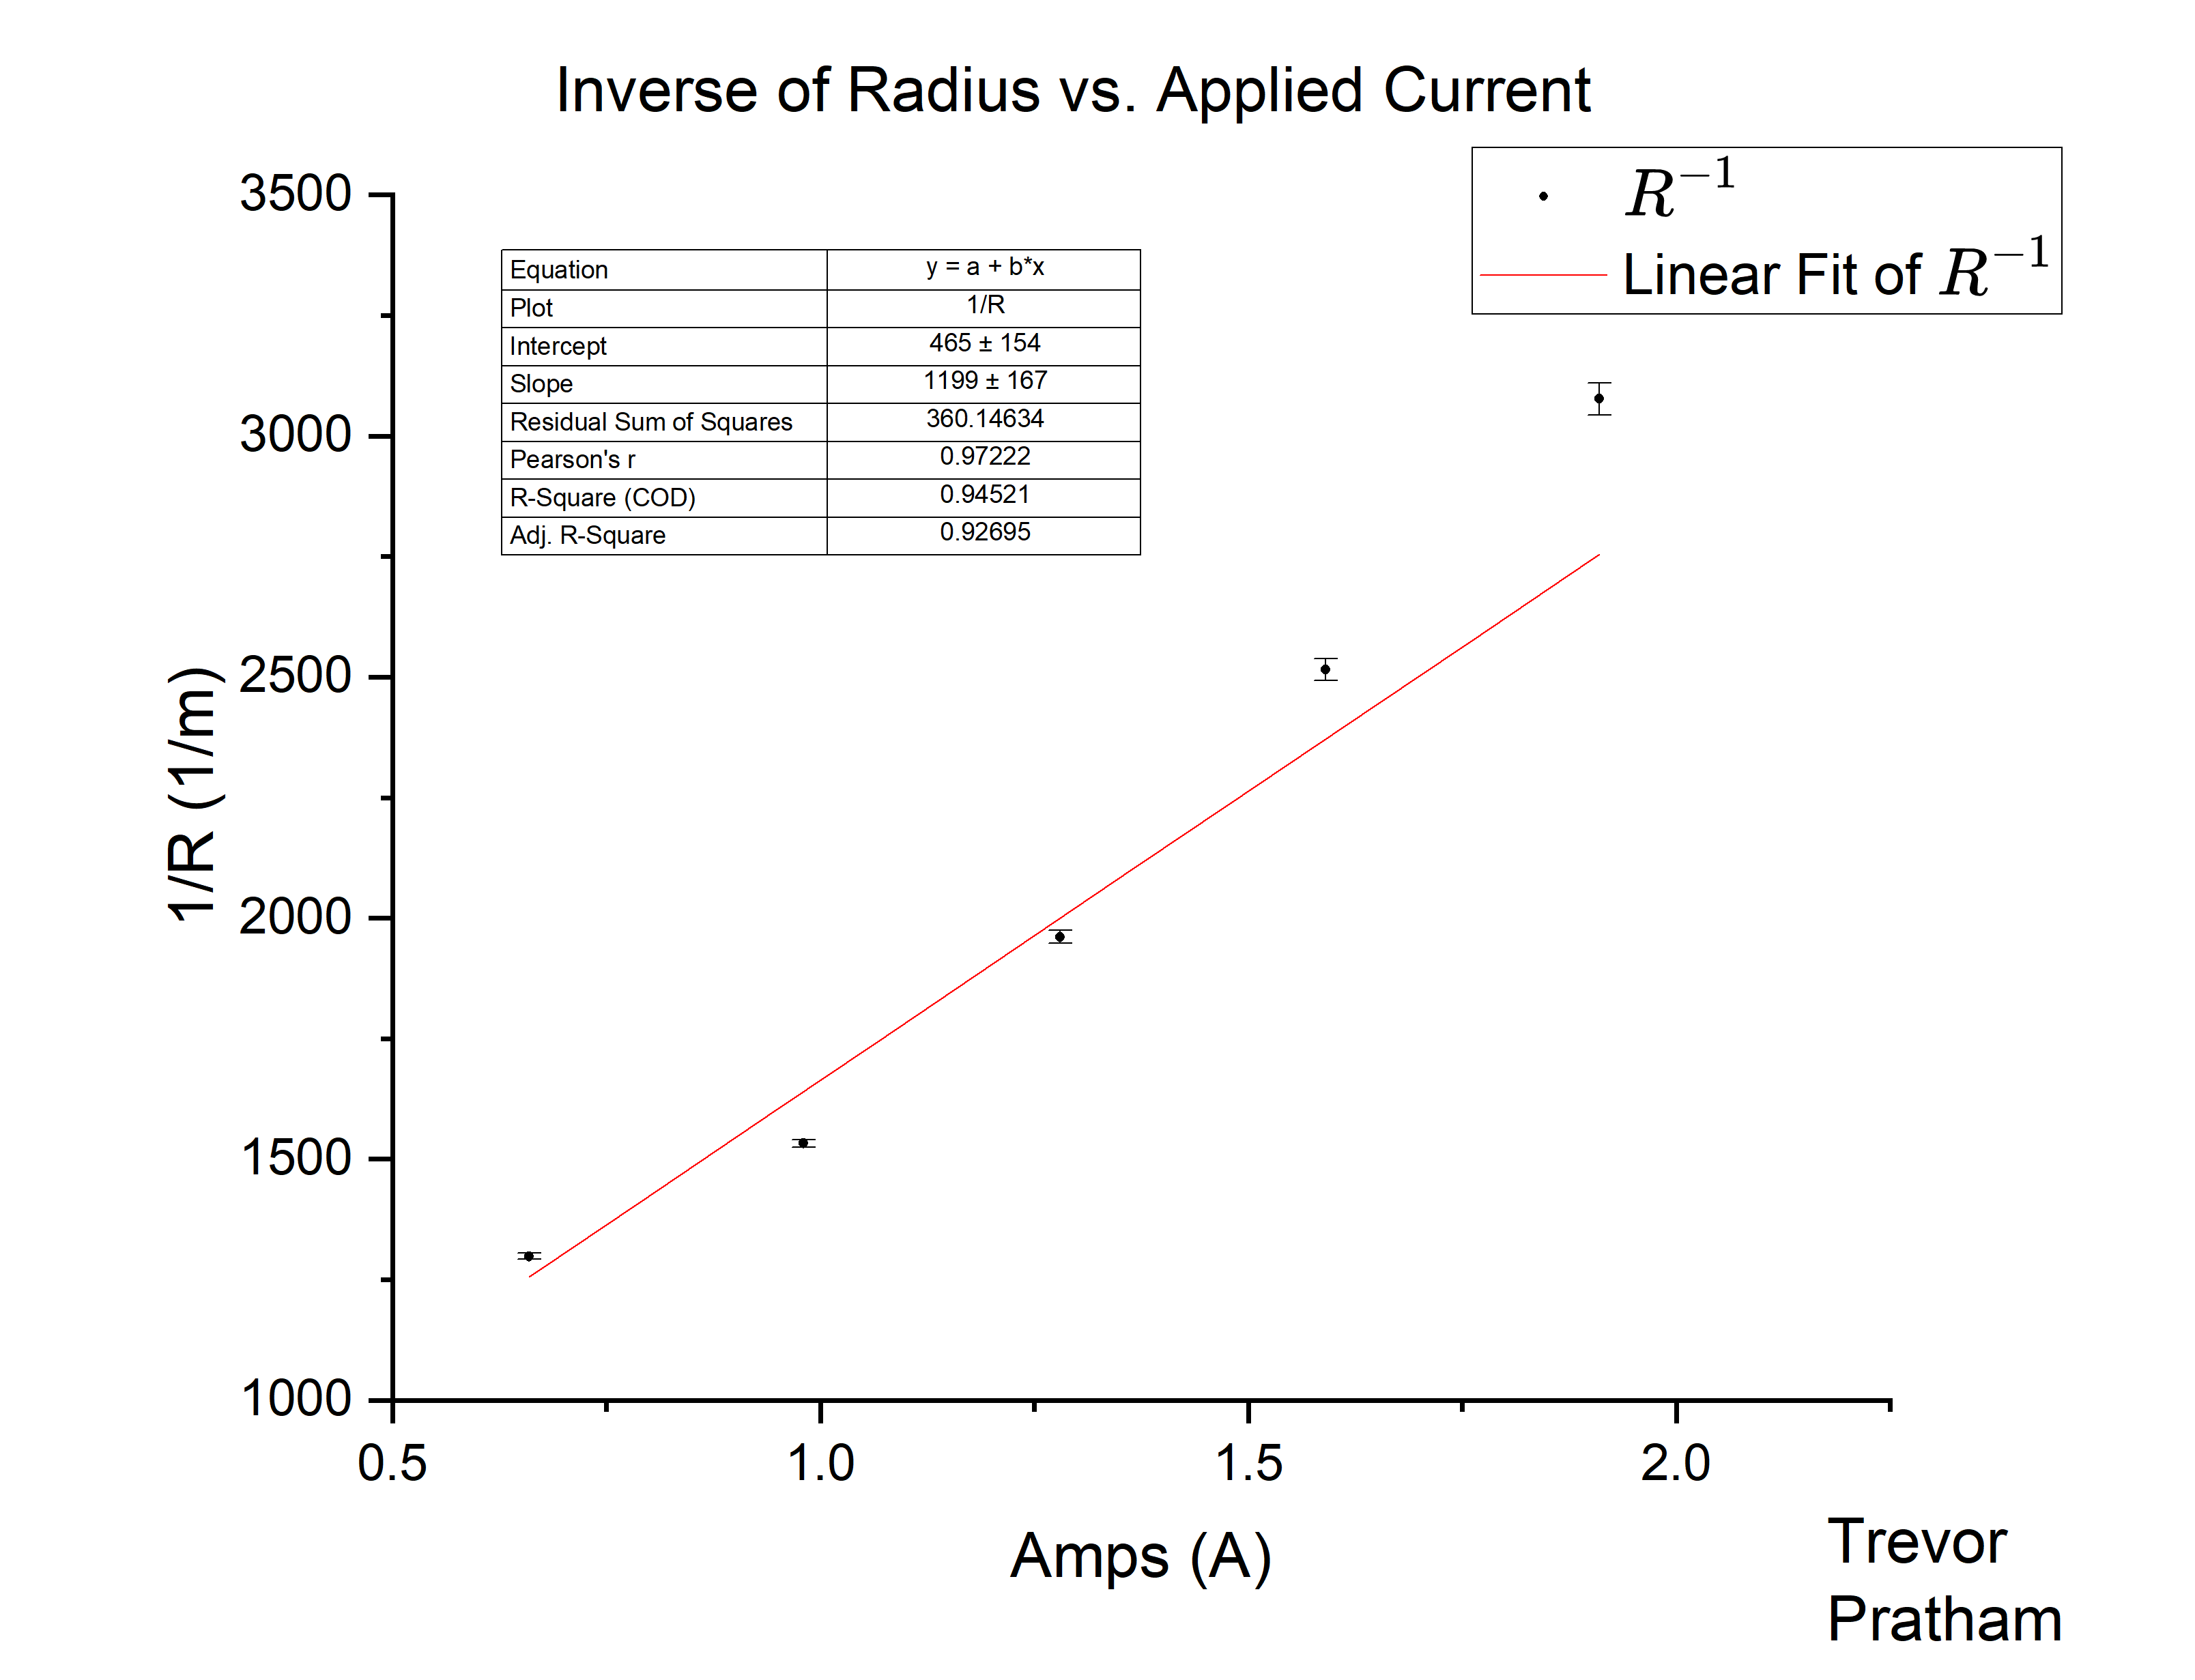
\includegraphics[width=0.7\textwidth]{figures/EOM_Fix_Voltage.png}
        \caption{Inverse of radius $\frac{1}{R}$ vs. applied current $A$. 1/R is calculated as 1 over the Average Radius values reported in Table \ref{t_FixV}.}
        \label{p_FixV}
    \end{subfigure}
\end{figure}

\clearpage

\subsection{Fixed Amps Data and Figures}

\begin{table}[h]
    \centering
    \begin{tabular}{|c|c|c|c|}
        \hline
        Voltage & Trevor's D (cm) & Pratham's D (cm) & Average Radius (m) \\ 
        \hline
        84 & 10.4 $\pm$ 0.1 & 10.3 $\pm$ 0.1 & 5.175E-4 $\pm$ 3.5E-6 \\ 
        113 & 11.8 $\pm$ 0.1 & 12.5 $\pm$ 0.1 & 6.075E-4 $\pm$ 3.5E-6 \\ 
        139 & 14.4 $\pm$ 0.1 & 13.7 $\pm$ 0.1 & 7.025E-4 $\pm$ 3.5E-6 \\ 
        168 & 15.2 $\pm$ 0.1 & 14.8 $\pm$ 0.1 & 7.500E-4 $\pm$ 3.5E-6 \\
        197 & 15.8 $\pm$ 0.1 & 15.5 $\pm$ 0.1 & 7.825E-4 $\pm$ 3.5E-6 \\
        \hline
    \end{tabular}
    \caption{Fixed Amps at $A = 1.02\pm0.01 A$, with steps of voltage from a minimum Voltage of $84V$ and a maximum of $197V$. Trevor's and Pratham's D refers to their measured diameter values, respectively. The Average Radius Values and Uncertainties here are identical to the values calculated Table \ref{t_FixV}. See the next section for uncertainty discussions.}
    \label{t_FixA}
\end{table}

\begin{figure} [h]
    \begin{subfigure}
        \centering
        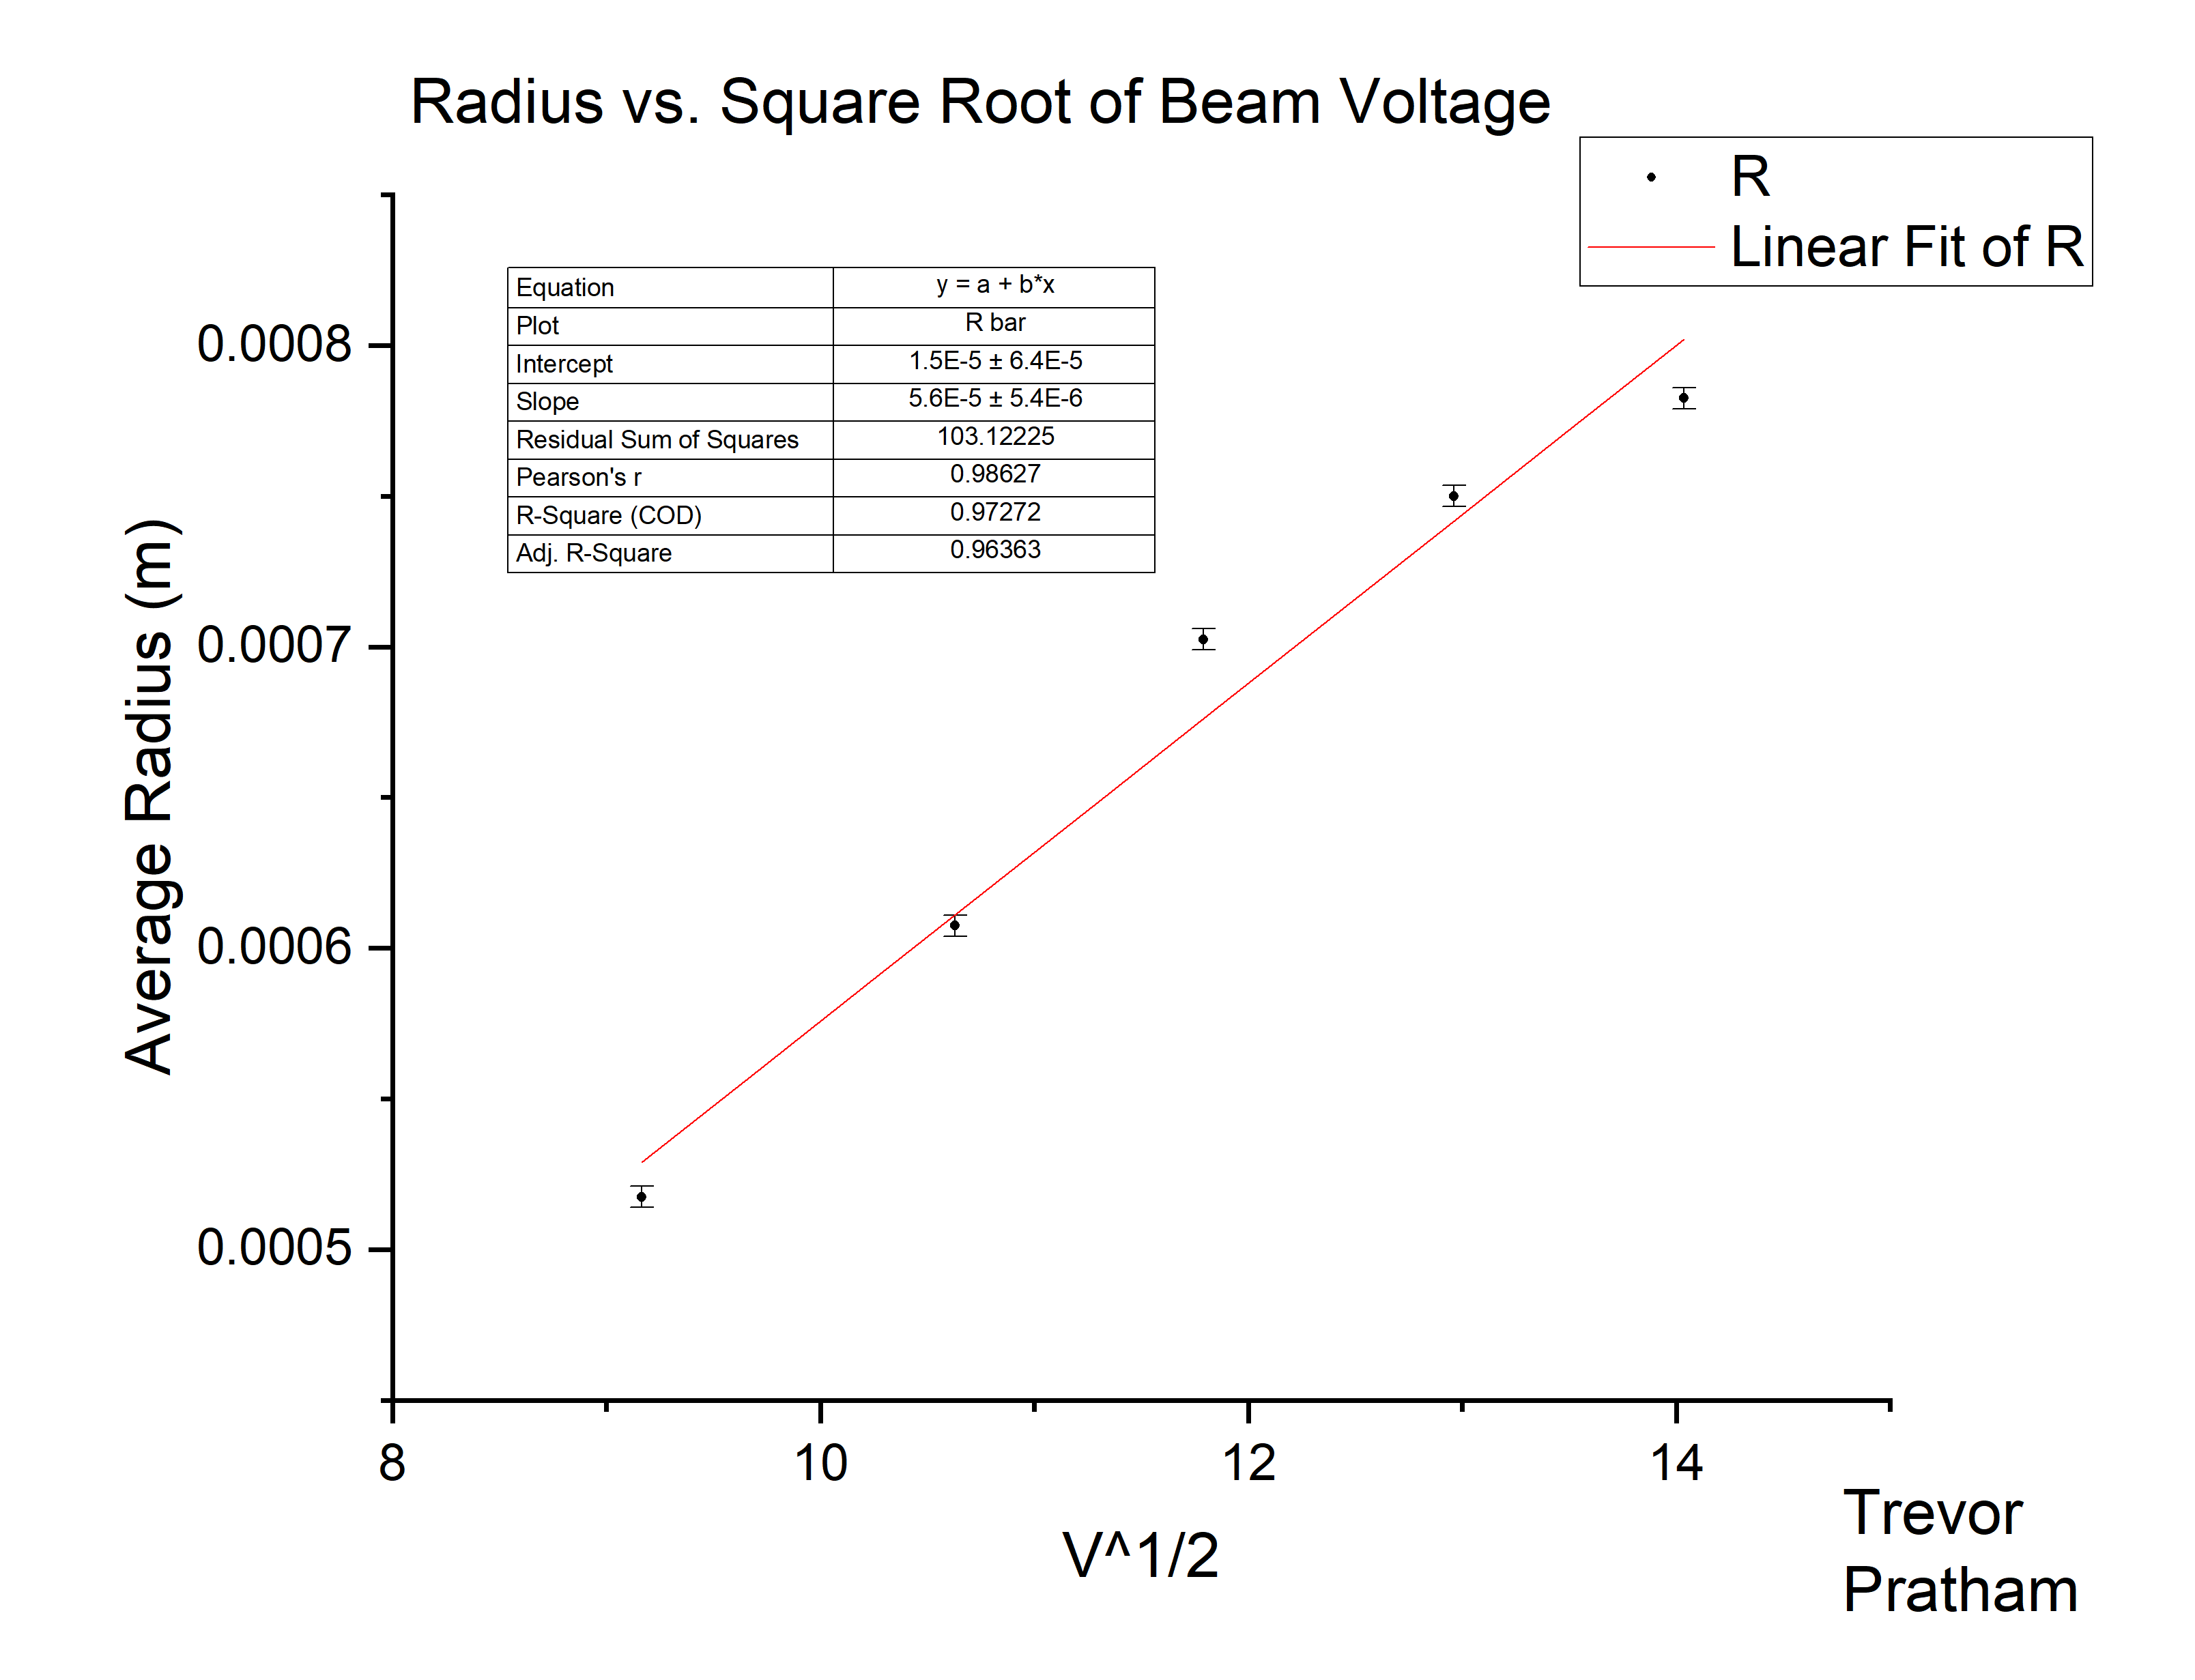
\includegraphics[width=0.7\textwidth]{figures/EOM_Fix_Amps.png}
        \caption{Radius $R$ vs. applied beam voltage $V$}
        \label{p_FixA}
    \end{subfigure}
\end{figure}

\clearpage

\section{Other Calculations}
\subsection{Average Radius Error Propagation} \label{sec:RadiusErr}

\begin{align*}
	\bar{R} =& \frac{1}{2}\cdot\frac{D_T + D_P}{2}\cdot\frac{1 m}{100 cm} = \frac{1}{400}\cdot(D_T + D_P)\ m && \text{for diameter measurements }D_T \text{ and }D_P \\
	\delta_{\bar{R}} =& \sqrt{\delta_{\bar{R}_{D_T}}^2 + \delta_{\bar{R}_{D_P}}^2} && \text{errors present only in }D_T \text{ and }D_P \\
	\delta_{\bar{R}_{D_T}} =& \left( \frac{\partial \bar{R}}{\partial D_T} \right)\cdot\delta_{D_T} = \frac{1}{400}\cdot\delta_{D_T} && \text{use }\delta_{D_T}=0.001\text{ m -- from measurements} \\
	=& \frac{1}{400}\cdot0.001=2.5\times10^{-6} m \\
	\delta_{\bar{R}_{D_T}} =& \left( \frac{\partial \bar{R}}{\partial D_P} \right)\cdot\delta_{D_P} = \frac{1}{400}\cdot\delta_{D_P} && \text{use }\delta_{D_P}=0.001\text{ m -- from measurements} \\
	=& \frac{1}{400}\cdot0.001=2.5\times10^{-6} m \\
	\therefore \delta_{\bar{R}} =& \sqrt{(2.5\times10^{-6}m)^2+ (2.5\times10^{-6}m)^2} = 3.5\times10^{-6} m
\end{align*}

\begin{equation}
	\delta_{\bar{R}} = 3.5\times10^{-6} m
	\label{R_bar_err}
\end{equation}

\subsection{Error Propagation in 1/R} \label{sec:InvRadiusError}

\begin{align*}
	\frac{1}{\bar{R}}=& \frac{1}{R} && \text{Used for determining }\alpha \\
	\delta_{\frac{1}{\bar{R}}} =& \delta_{\frac{1}{\bar{R}}_{\bar{R}}} && \text{No need for adding in quadrature, only once source of error} \\
	\delta_{\frac{1}{\bar{R}}_{\bar{R}}} =& \abs{\paren{\frac{\partial \frac{1}{\bar{R}}}{\partial \bar{R}}}\cdot\delta_{\bar{R}}} && \text{Derivative method for error propagation} \\
	=& \frac{\delta_{\bar{R}}}{\bar{R}^2} && \text{Simple single-variable derivative}
\end{align*}

This expression was used in determining the errors presented in Table \ref{t_FixV}, but calculations are omitted here to prevent redundancy. To calculate, use $\delta_{\bar{R}}=3.5\times10^{-6} m$, as calculated in the above subsection.

\begin{equation}
	\delta_{\frac{1}{\bar{R}}}=\frac{\delta_{\bar{R}}}{\bar{R}^2}
	\label{R_bar_inverse_err}
\end{equation}

\clearpage

\subsection{Hemholtz Coil Current Error Propagation - Fixed Voltage} \label{sec:FixedVoltageErr}

\begin{equation}
	\alpha = \frac{8\mu_0N}{5r}\sqrt{\frac{e/m}{10V}}\
	\quad \Rightarrow \quad
	\frac{e}{m}=\paren{\frac{5r\alpha}{8\mu_0N}}^2\cdot(10V)
	\quad \text{Errors propagated in }\alpha, V, r 
	\label{em_derive_FixV}
\end{equation}

\begin{align*}
	\delta_\frac{e}{m}=&\sqrt{\paren{\delta_{\frac{e}{m}_\alpha}}^2+\paren{\delta_{\frac{e}{m}_V}}^2+\paren{\delta_{\frac{e}{m}_r}}^2} && \text{General Error Equation} \\ \\
	\delta_{\frac{e}{m}_\alpha} = \paren{\frac{\partial \frac{e}{m}}{\partial \alpha}}\cdot\delta_\alpha =& \paren{20\paren{\frac{5}{8\mu_0N}}^2(r\alpha^2)V}\cdot\delta_\alpha && \text{Error due to }\alpha \\
	=& \paren{20\paren{\frac{5}{8\cdot4\pi\times10^{-7}\cdot130}}^2(0.158\cdot1199^2)\cdot104}\cdot167 \\
	=& 1.15\times10^{18} \frac{C}{Kg} \\ \\
	\delta_{\frac{e}{m}_V} = \paren{\frac{\partial \frac{e}{m}}{\partial V}}\cdot\delta_V =& \paren{10\paren{\frac{5}{8\mu_0N}}^2(r^2\alpha^2)}\cdot \delta_V && \text{Error due to }V \\
	=& \paren{10\paren{\frac{5}{8\cdot4\pi\times10^{-7}\cdot130}}^2(0.158^2\cdot1199^2)}\cdot1 \\
	=& 5.25\times10^{12} \frac{C}{Kg} \\ \\
	\delta_{\frac{e}{m}_r} = \paren{\frac{\partial \frac{e}{m}}{\partial r}}\cdot\delta_r =& \paren{20\paren{\frac{5}{8\mu_0N}}^2(r^2\alpha)V}\cdot \delta_r && \text{Error due to }r \\
	=& \paren{20\paren{\frac{5}{8\cdot4\pi\times10^{-7}\cdot130}}^2(0.158^2\cdot1199)\cdot104}\cdot0.005 \\
	=& 4.38\times10^7 \frac{C}{Kg} \\ \\
	\delta_\frac{e}{m} =& \sqrt{(1.15\times10^{18})^2+(5.25\times10^{12})^2+(4.38\times10^7)^2} && \text{Substitute Values}\\
	=& 1.15\times10^{18} \frac{C}{Kg}
\end{align*}

\clearpage

\subsection{Beam Voltage Error Propagation - Fixed Amps} \label{sec:FixedAmpsErr}

\begin{equation}
	\beta = \frac{5r}{8\mu_0N I_c}\sqrt{\frac{10}{e/m}}
	\quad \Rightarrow \quad
	\frac{e}{m}=10\paren{\frac{8\mu_0N I_C\beta}{5r}}^{-2}
	\quad \text{Errors propagated in }\beta, I_c, r
	\label{em_derive_FixA}
\end{equation}

\begin{align*}
	\delta_\frac{e}{m}=&\sqrt{\paren{\delta_{\frac{e}{m}_\beta}}^2+\paren{\delta_{\frac{e}{m}_{I_c}}}^2+\paren{\delta_{\frac{e}{m}_r}}^2} \\ \\
	\delta_{\frac{e}{m}_\beta} = \abs{\paren{\frac{\partial \frac{e}{m}}{\partial \beta}}\cdot\delta_\beta} =& \paren{\paren{\frac{8\mu_0N}{5}}^{-2}\cdot\paren{\frac{20r^2}{\beta^3I_c^2}}}\cdot\delta_\beta \\
	=& \paren{\paren{\frac{8\cdot4\pi\times10^{-7}*130}{5}}^{-2}\cdot\paren{\frac{20(0.158)^2}{(5.6\times10^{-5})^3(1.02)^2}}}\cdot(5.4\times10^{-6}) \\
	=& 2.16\times10^{14} \frac{C}{Kg} \\ \\
	\delta_{\frac{e}{m}_{I_c}} = \abs{\paren{\frac{\partial \frac{e}{m}}{\partial I_c}}\cdot\delta_{I_c}} =& \paren{\paren{\frac{8\mu_0N}{5}}^{-2}\cdot\paren{\frac{20r^2}{\beta^2I_c^3}}}\cdot \delta_{I_c} \\
	=& \paren{\paren{\frac{8\cdot4\pi\times10^{-7}*130}{5}}^{-2}\cdot\paren{\frac{20(0.158)^2}{(5.6\times10^{-5})^2(1.02)^3}}}\cdot0.01\\
	=& 2.20\times10^{13} \frac{C}{Kg} \\ \\
	\delta_{\frac{e}{m}_r} = \abs{\paren{\frac{\partial \frac{e}{m}}{\partial r}}\cdot\delta_r} =& \paren{\paren{\frac{8\mu_0N}{5}}^{-2}\cdot\paren{\frac{20r}{\beta^2I_c^2}}}\cdot \delta_r \\
	=& \paren{\paren{\frac{8\cdot4\pi\times10^{-7}*130}{5}}^{-2}\cdot\paren{\frac{20(0.158)}{(5.6\times10^{-5})^2(1.02)^2}}}\cdot0.005 \\
	=& 1.42\times10^{14} \frac{C}{Kg} \\ \\
	\delta_\frac{e}{m} =& \sqrt{(2.16\times10^{14})^2+(2.20\times10^{13})^2+(1.42\times10^{14})^2} \\
	=& 2.59\times10^{14} \frac{C}{Kg}
\end{align*}

\end{document}
